\documentclass[french,a4paper,addpoints,11pt]{exam}
\usepackage{hexercises-series}
\usepackage{mathtools, nccmath}
\usepackage{tabularx}
\title{Structure de données récursives}
\seriesno{\texttt{0x28}}
\department{TIN}
\classroom{INFO2-TIN}

\begin{document}
\maketitle

\ifprintanswers
\else
\begin{multicols}{2}
\fi

\begin{questions}

\question On considère une liste simplement chaînée dont chaque noeud peut contenir un `float`. La liste est caractérisée par deux structures \CD{Node} et \CD{List}.

\begin{parts}
\part Implémentez le type \CD{Node} et la définition de son contenu.

\begin{solution}
\begin{lstlisting}
typedef struct node {
  double value;
  struct node *next;
} Node;
\end{lstlisting}
\end{solution}

\part Implémentez le type \CD{List} et la définition de son contenu. Cette dernière permet d'accéder le premier et le dernier élément de la liste et contient également le nombre d'éléments dans la liste.

\begin{solution}
\begin{lstlisting}
typedef struct list {
  size_t count;
  Node *head;
  Node *tail;
} Node;
\end{lstlisting}
\end{solution}

\part Implémentez la fonction \CD{push} permettant d'insérer un nouvel élément dans la liste. Veillez aux cas particuliers, par exemple lorsque la liste est vide. La fonction retourne une valeur négative en cas d'erreur, zéro en cas de succès.

\begin{solution}
\begin{lstlisting}
int push(List *list, double value) {
  Node *node = malloc(sizeof(Node));
  if (node == NULL) {
    return -1;
  }
  node->value = value;
  node->next = NULL;
  if (list->count == 0) {
    list->head = node;
    list->tail = node;
  } else {
    list->tail->next = node;
    list->tail = node;
  }
  list->count++;
  return 0;
}
\end{lstlisting}
\end{solution}

\part Implémentez la fonction \CD{mean} permettant de calculer la valeur moyenne du contenu de la liste.

\begin{solution}
\begin{lstlisting}
double mean(List *list) {
  double sum = 0;
  Node *node = list->head;
  while (node != NULL) {
    sum += node->value;
    node = node->next;
  }
  return sum / list->count;
}
\end{lstlisting}
\end{solution}

\part Implémentez une fonction de comparaison \CD{compare} qui reçoit deux listes et retourne 0 si le contenu est identique, et 1 sinon.

\begin{solution}
\begin{lstlisting}
int compare(List *a, List *b) {
  if (a->count != b->count) {
    return -1;
  }
  Node *node_a = a->head;
  Node *node_b = b->head;
  while (node_a != NULL) {
    if (node_a->value != node_b->value) {
      return -1;
    }
    node_a = node_a->next;
    node_b = node_b->next;
  }
  return 0;
}
\end{lstlisting}
\end{solution}
\end{parts}

\question Un BST (\emph{Binary Search Tree}) est un arbre binaire respectant la propriété suivante : l'enfant de gauche est toujours plus petit que son parent et l'enfant de droite est toujours plus grand que son parent. Voici un exemple :

\begin{center}
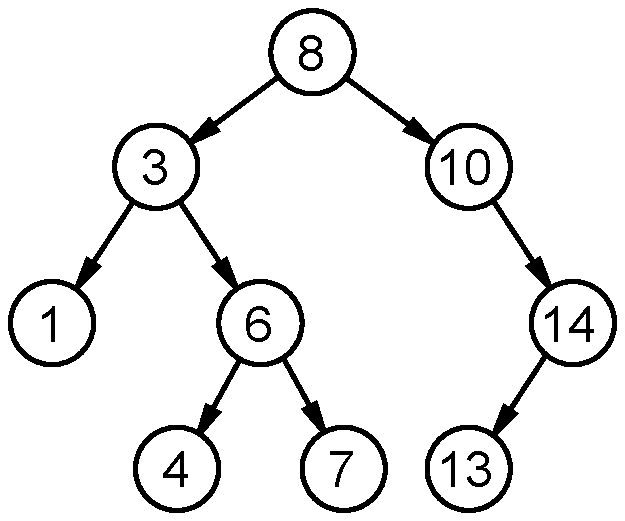
\includegraphics[width=6cm]{assets/bst.pdf}
\end{center}

Cette question porte sur cet arbre binaire de recherche.

\begin{parts}
\part Écrire la structure de donnée d'un noeud d'un BST contenant des valeurs entières non signées.

\begin{solution}
\begin{lstlisting}
typedef struct node {
  unsigned int value;
  struct node *left;
  struct node *right;
} Node;
\end{lstlisting}
\end{solution}

\part Écrire une fonction récursive permettant de rechercher une valeur dans un bst. Si la valeur est trouvée la fonction retourne 1, sinon 0.

\begin{solution}
\begin{lstlisting}
int search(Node *root, unsigned int value) {
  if (root == NULL) return 0;
  if (root->value == value) return 1;
  return search(
    root->value > value ? root->left : root->right, value);
}
\end{lstlisting}
\end{solution}

\part Quelle est la complexité en temps (Big-O) pour la recherche d'un élément dans un BST ?

\begin{solution}
$O(\log n)$
\end{solution}
\end{parts}
\end{questions}
\ifprintanswers
\else
\end{multicols}
\fi
\end{document}
